\documentclass[11pt]{article}
\usepackage[margin=2.2cm]{geometry}
\usepackage{graphicx}
\usepackage{hyperref}
\usepackage{booktabs}
\usepackage{xcolor}
\hypersetup{colorlinks=true, linkcolor=blue, urlcolor=blue, citecolor=blue}

% small single-color frequency-coverage thumbnail for one pulsar + one
% CASE_STYLE entry -- generated by summary/make_color_key_thumbnails.py
\newcommand{\keyplot}[2]{\includegraphics[width=2.1cm]{assets/key_#1_#2.pdf}}
% the full 11-case color key (all 6 datasets x up to 2 models), using #1's
% own data -- used once in the Overview (J1744-1134, as a shared example)
% and once per pulsar section (that pulsar's own data) right before its
% corner-plot comparisons. Not isolated by station-set split (2026-10-30):
% every comparison below, including the lofaronly ones, lives in one
% "Noise-model comparisons" subsection per pulsar, so one combined key
% covers all of them.
\newcommand{\colorkeytable}[1]{%
  \begin{center}
  \renewcommand{\arraystretch}{1.3}
  \begin{tabular}{l c c}
  \toprule
   & \textbf{DM+RN} (solid) & \textbf{RN only} (dashed) \\
  \midrule
  combined, corrected    & \keyplot{#1}{caseCorrDMRN}   & \keyplot{#1}{caseCorrRN}   \\
  highfreq, corrected    & \keyplot{#1}{caseHFDMRN}     & \keyplot{#1}{caseHFRN}     \\
  lofaronly, corrected   & \keyplot{#1}{caseLoCorrDMRN} & \keyplot{#1}{caseLoCorrRN} \\
  combined, uncorrected  & \keyplot{#1}{caseUncDMRN}    & \keyplot{#1}{caseUncRN}    \\
  highfreq, uncorrected  & --                           & \keyplot{#1}{caseHFURN}    \\
  lofaronly, uncorrected & \keyplot{#1}{caseLoUncDMRN}  & \keyplot{#1}{caseLoUncRN}  \\
  \bottomrule
  \end{tabular}
  \end{center}
}

\title{DM(t) Correction from LOFAR: Noise-Analysis Summary}
\author{De\_coloring project}
\date{\today}

% Comparisons as inline graphics (not \includepdf, which forces one page per
% file even when the content is a small 2x2 corner-plot grid -- that left
% every comparison on its own mostly-empty page). No forced page breaks here,
% so LaTeX packs several comparisons per page on its own. Each block is a
% minipage so it cannot itself be split across a page boundary (caption and
% images always stay together, pushed to the next page as a unit if needed).
%
% \cmpjoint: a joint RN+DM corner (4x4), from compare_posteriors.py --joint.
% \cmpone: a rednoise-only corner (2x2), for comparisons of rnonly runs only.
\newcommand{\cmpjoint}[2]{%
  \noindent\begin{minipage}{\textwidth}
  \centering
  \textbf{\footnotesize #2}\par\vspace{2pt}
  \includegraphics[width=0.62\textwidth]{#1}%
  \end{minipage}\par\vspace{8pt}
}
\newcommand{\cmpone}[2]{%
  \noindent\begin{minipage}{\textwidth}
  \centering
  \textbf{\footnotesize #2}\par\vspace{2pt}
  \includegraphics[width=0.5\textwidth]{#1}%
  \end{minipage}\par\vspace{8pt}
}
% a single wide (not square) plot, e.g. the DM(t) time-series overlay
\newcommand{\cmpwide}[2]{%
  \noindent\begin{minipage}{\textwidth}
  \centering
  \textbf{\footnotesize #2}\par\vspace{2pt}
  \includegraphics[width=0.85\textwidth]{#1}%
  \end{minipage}\par\vspace{8pt}
}

\begin{document}
\maketitle
\tableofcontents

\section{Overview}

Three LOFAR-monitored MSPs (J1012+5307, J1640+2224, J1744$-$1134) have their
dispersion-measure variations measured directly from LOFAR data (epoch-wise
total-DM fits, smoothed with a Mat\'ern-3/2 GP), and this DM(t) curve is used
to correct the high-frequency TOAs over the LOFAR-constrained time span. The
question this summary addresses: once that correction is applied, does a
Bayesian noise analysis still want a stochastic DM-noise term, or does the
correction already remove it?

Six Tspan-matched feather datasets exist per pulsar (same time span, the
raw LOFAR coverage window), split along two axes --- station set and
correction status:
\begin{itemize}
  \item \textbf{highfreq\_corrected} --- high-frequency stations only (GMRT
    included, LOFAR/NenuFAR excluded), DM(t)-corrected;
  \item \textbf{highfreq\_uncorrected} --- high-frequency stations only,
    \emph{not} corrected;
  \item \textbf{lofaronly\_corrected} --- LOFAR/NenuFAR only, DM(t)-corrected;
  \item \textbf{lofaronly\_uncorrected} --- LOFAR/NenuFAR only, \emph{not}
    corrected;
  \item \textbf{combined\_corrected} --- every station, DM(t)-corrected;
  \item \textbf{combined\_uncorrected} --- every station, \emph{not}
    corrected (NE\_SW $\to$ 0, DM1/DM2 left free) --- the reference.
\end{itemize}
\textbf{highfreq\_corrected} + \textbf{lofaronly\_corrected} =
\textbf{combined\_corrected} (same TOAs, same correction, just split by
station set), and likewise for the uncorrected triple. Each pulsar's
``Noise-model comparisons'' subsection below overlays all three station
splits together wherever that is informative (e.g.\ \emph{highfreq} vs
\emph{lofaronly} vs \emph{combined}, same correction status and model, as a
single three-way corner) rather than keeping \emph{lofaronly} isolated in
its own section -- the station-set split is one more axis to compare, not a
separate analysis.

Two noise models (jexplore, default priors): \textbf{rnonly} (white noise +
ECORR on LOFAR/NenuFAR/DE60x + achromatic red noise, 30 Fourier components)
and \textbf{dmrn} (rnonly + a DM GP, 100 components, powerlaw PSD). The two
stochastic Gaussian processes compared throughout this document:

\begin{center}
\renewcommand{\arraystretch}{1.3}
\begin{tabular}{l c c c c c}
\toprule
\textbf{GP} & basis & PSD & components & $\log_{10}A$ prior & $\gamma$ prior \\
\midrule
rednoise (RN) & achromatic & powerlaw & 30  & $[-18, -11]$ & $[0, 7]$ \\
dmgp (DM)     & dm         & powerlaw & 100 & $[-18, -11]$ & $[0, 7]$ \\
\bottomrule
\end{tabular}
\end{center}

Every comparison plot in this document uses the same colorblind-safe
(Okabe--Ito) convention: the \emph{color} identifies the dataset, the
\emph{line style} the noise model --- solid for DM+RN, dashed for RN only.
Contours are drawn at $1\sigma$ and $2\sigma$. A color-key table (each cell
a small frequency-vs-MJD thumbnail of that pulsar's own data, in that
dataset's color, with a dashed frame for RN only) opens each pulsar's
noise-model-comparisons section below.

\section{J1012+5307}
\label{sec:J1012}

\subsection{Epoch-wise DM(t) correction}
\begin{center}
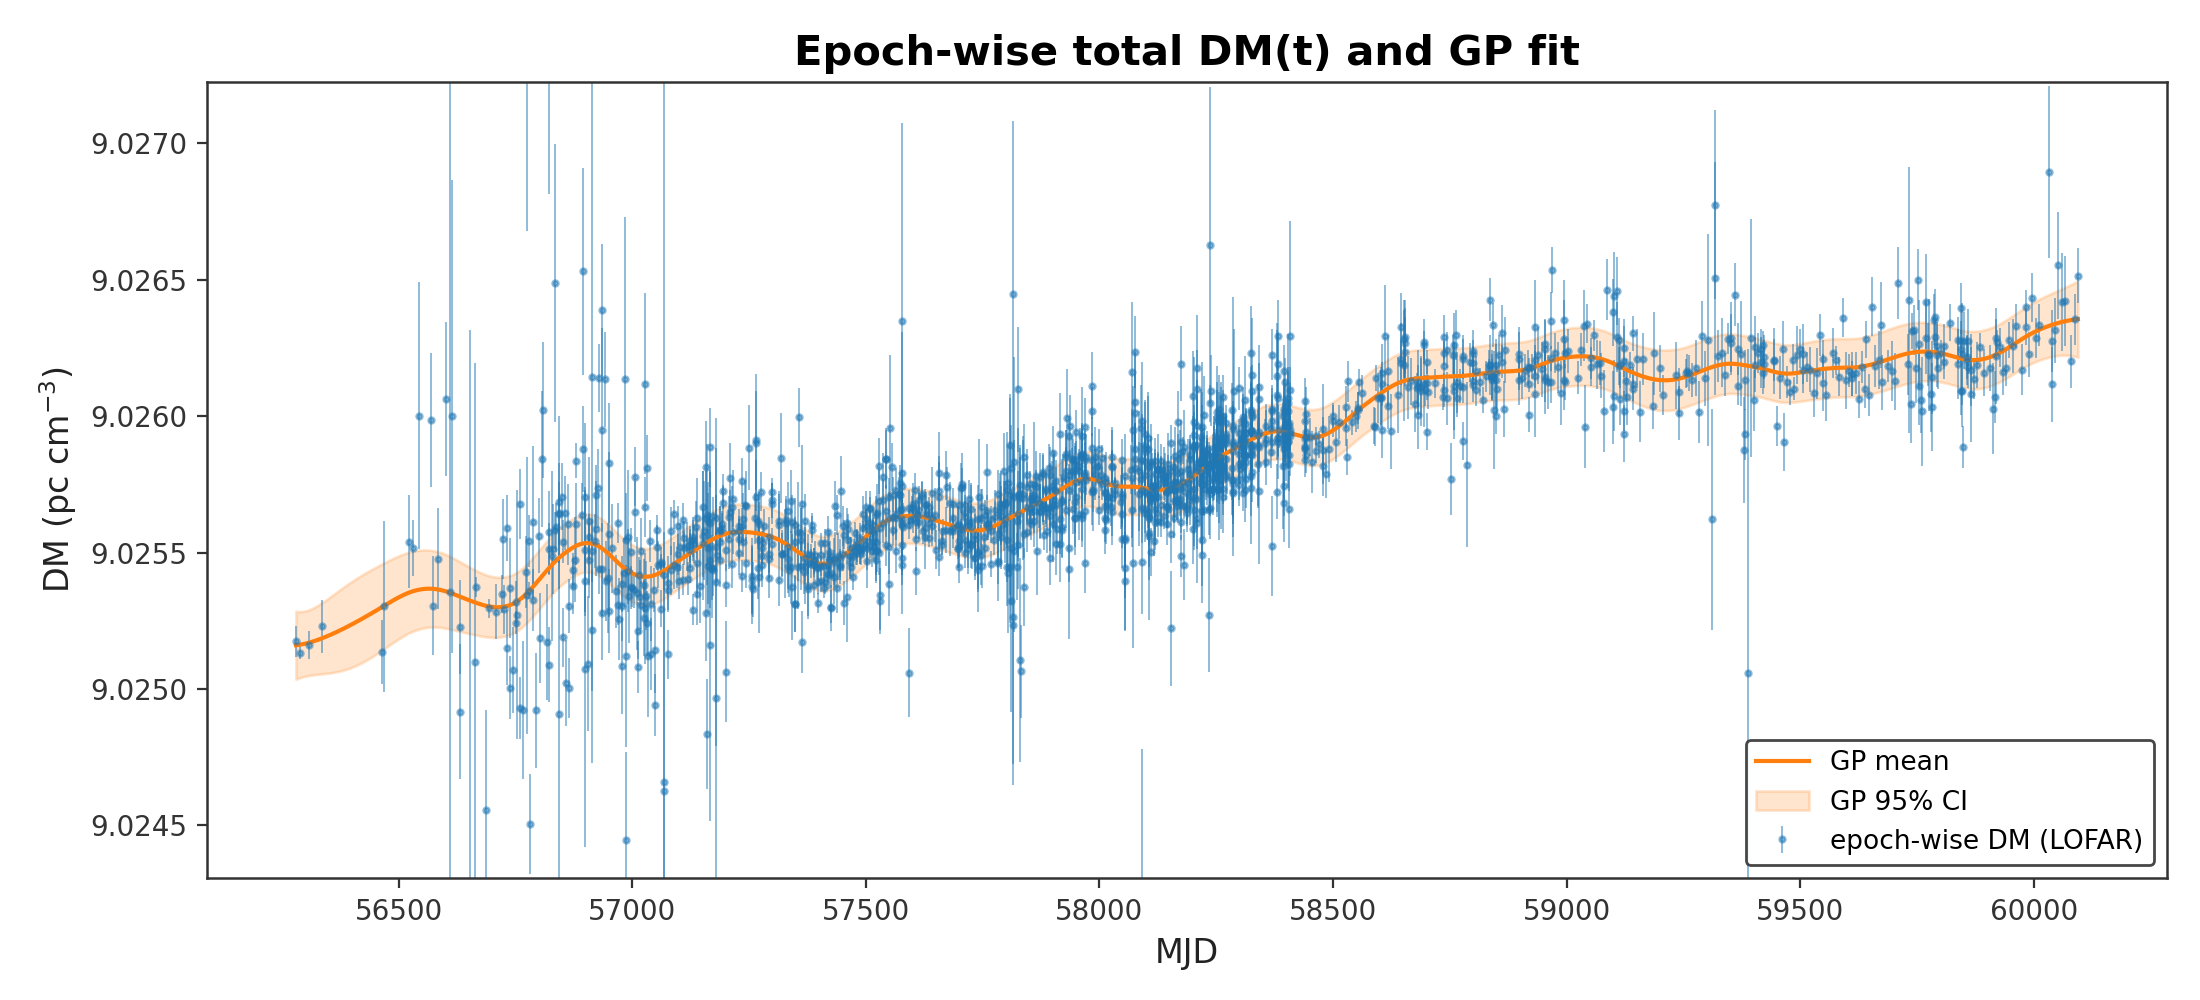
\includegraphics[width=0.8\textwidth]{../J1012+5307/dm_correction_out/dm_timeseries.png}
\end{center}

\subsection{Effect on residuals}
\begin{center}
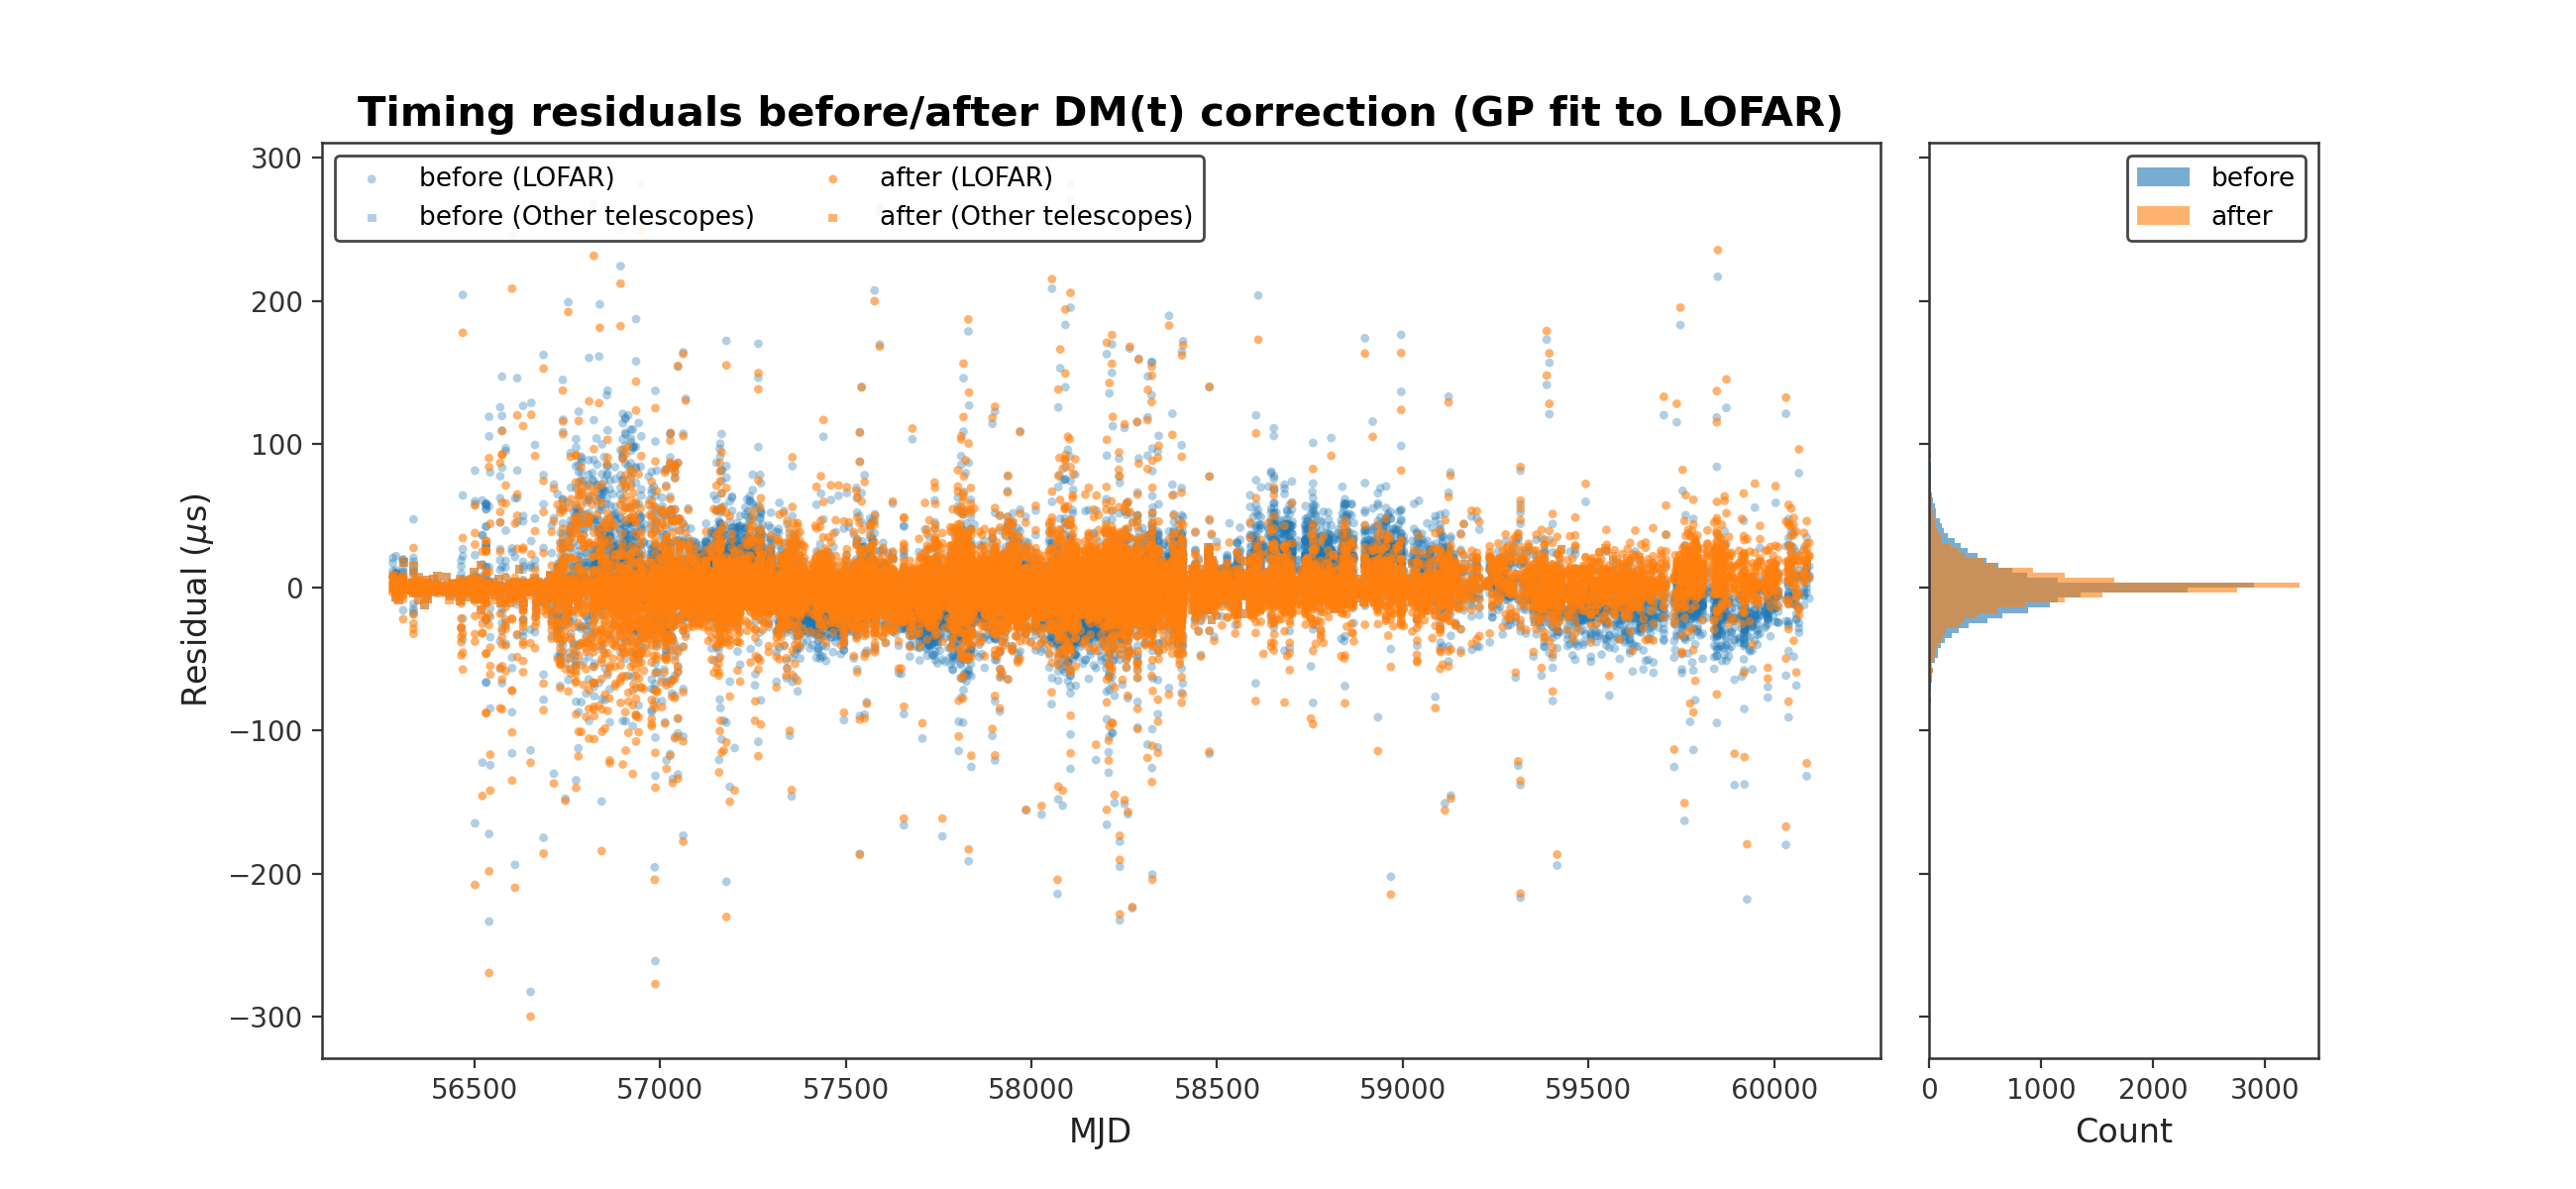
\includegraphics[width=0.8\textwidth]{../J1012+5307/dm_correction_out/residuals_pre_post.png}
\end{center}

\subsection{Noise-model comparisons}

\colorkeytable{J1012+5307}

\cmpjoint{../plot_output/compare/J1012+5307.pdf}{highfreq\_corrected: rnonly vs dmrn}
\cmpjoint{../plot_output/compare/J1012+5307_lofaronly_corrected_rnonly_vs_dmrn.pdf}{lofaronly\_corrected: rnonly vs dmrn}
\cmpjoint{../plot_output/compare/J1012+5307_corrected_dmrn_3way.pdf}{corrected, dmrn: highfreq vs lofaronly vs combined}
\cmpone{../plot_output/compare/J1012+5307_rnonly_combined_vs_highfreq.pdf}{corrected, rnonly: combined vs highfreq (lofaronly omitted --- see caveat below)}
\cmpjoint{../plot_output/compare/J1012+5307_uncorrected_vs_corrected.pdf}{combined: uncorrected vs corrected (dmrn)}
\cmpjoint{../plot_output/compare/J1012+5307_lofaronly_corr_vs_uncorr_dmrn.pdf}{lofaronly: corrected vs uncorrected (DM+RN)}
\cmpone{../plot_output/compare/J1012+5307_lofaronly_corr_vs_uncorr_rnonly.pdf}{lofaronly: corrected vs uncorrected (RN only)}
\cmpjoint{../plot_output/compare/J1012+5307_rnonly-corrected_vs_dmrn-uncorrected.pdf}{combined\_corrected:rnonly vs combined\_uncorrected:dmrn}
\cmpjoint{../plot_output/compare/J1012+5307_lofaronly_uncorrected_rnonly_vs_dmrn.pdf}{lofaronly\_uncorrected: rnonly vs dmrn}
\cmpone{../plot_output/compare/J1012+5307_rnonly_highfreqU_vs_lofaronlyU_vs_combinedU.pdf}{RN only, uncorrected: highfreq vs lofaronly vs combined}

\subsection{DM(t): GP reconstruction vs epoch-wise}
\cmpwide{../plot_output/compare/J1012+5307_dm_timeseries_ew_vs_gp.pdf}{combined\_corrected:dmrn DM GP vs the original epoch-wise curve}

\subsection{Interpretation}

J1012+5307 is the known difficult case for this sampler (flagged in the
jexplore-noise devlog as multimodal, needing a denser temperature ladder) ---
its \emph{combined\_corrected:dmrn} run finished with only 23 total epochs,
so results here should be read with that caveat in mind. With that said, the
red noise found in \emph{combined} is systematically offset in both $\gamma$
and amplitude from \emph{highfreq} and from \emph{combined\_uncorrected:dmrn}'s
achromatic channel, with no overlap in any of the three comparisons. This is
the clearest non-coincidence of the three pulsars: whatever the correction is
leaving behind, it is enough to pull the red-noise fit to a different
solution whenever LOFAR is in the dataset without an explicit DM GP to
absorb it.

Splitting the corrected dataset by station set under \emph{dmrn} shows
\emph{combined} is not a simple blend of its two halves: all three settle
on their own distinct, mutually exclusive red-noise peak (lowest
$\gamma$/amplitude for \emph{highfreq}, highest for \emph{lofaronly},
\emph{combined} in between), and likewise for the DM GP --- \emph{lofaronly}'s
own DM GP rails to near-zero amplitude on its own (nothing obviously left
for it to find, consistent with the degeneracy test below), yet once
\emph{lofaronly} is merged into \emph{combined}, a modest but
well-determined DM GP peak emerges that neither sub-component shows alone.
(The equivalent \emph{rnonly} three-way plot is omitted here: J1012+5307's
\emph{combined\_corrected:rnonly} needed an unusually deep burn-in
[19 epochs, reviewed directly from its trace], which would leave
\emph{lofaronly\_corrected:rnonly} --- only 20 epochs total --- with just
one post-burn epoch of samples; the two-way \emph{combined} vs
\emph{highfreq} comparison above uses each side's own appropriate burn
instead.) Isolating \emph{lofaronly} entirely and switching the noise model
on/off reproduces the same reassignment degeneracy on a smaller scale: with
no DM GP, \emph{lofaronly}'s corrected/uncorrected red-noise posteriors are
both well-constrained but completely disjoint ($\gamma\approx4.5$--$5$ vs
$\gamma\approx2.5$); adding a DM GP leaves corrected's red noise unchanged
(its DM GP rails to zero) while uncorrected's collapses to unconstrained
and its DM GP absorbs a signal with nearly the same spectral index the
RN-only fit had assigned to red noise. The same pattern recurs in the
three-way \emph{rnonly} split among the three \emph{uncorrected} station
sets: three mutually exclusive, well-determined peaks tracking which
frequency band dominates --- not what genuine achromatic noise should look
like.

\section{J1640+2224}
\label{sec:J1640}

\subsection{Epoch-wise DM(t) correction}
\begin{center}
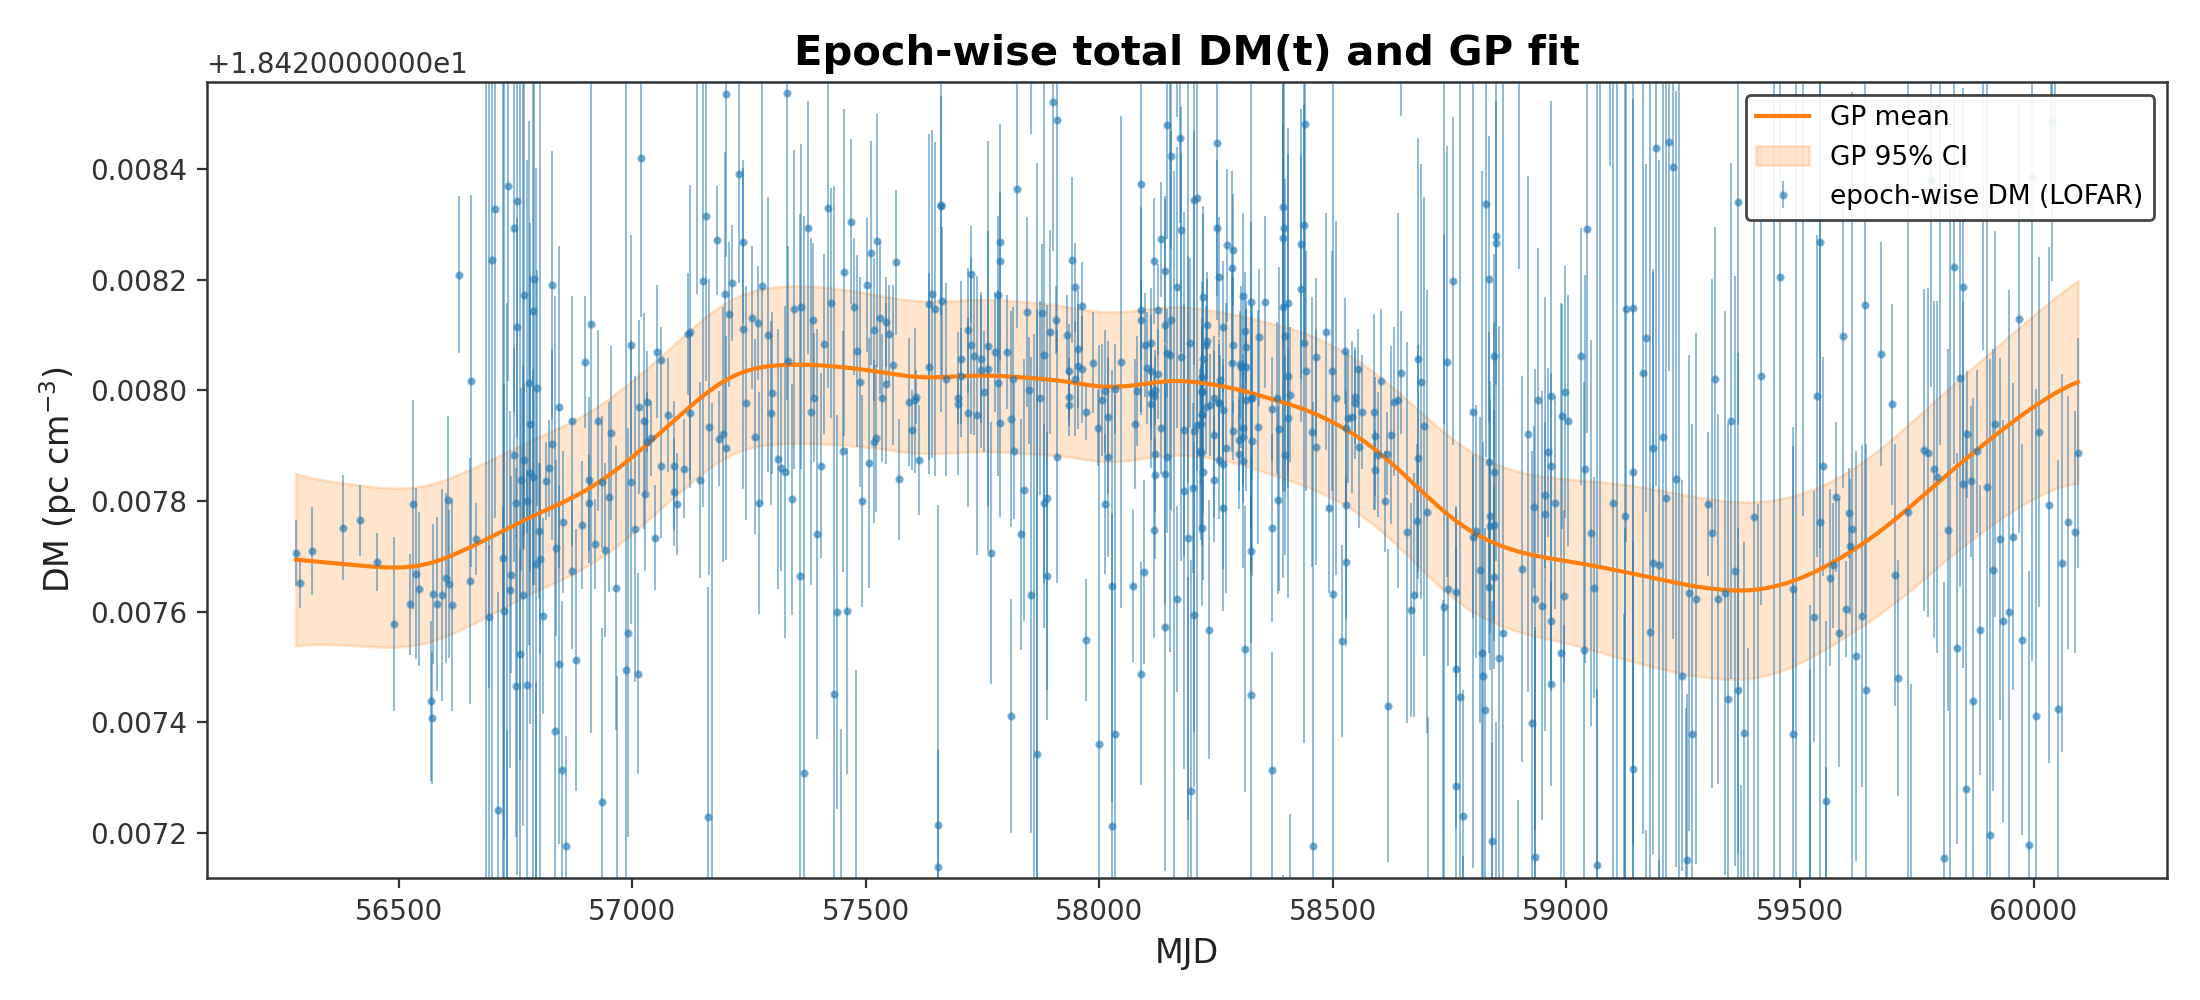
\includegraphics[width=0.8\textwidth]{../J1640+2224/dm_correction_out/dm_timeseries.png}
\end{center}

\subsection{Effect on residuals}
\begin{center}
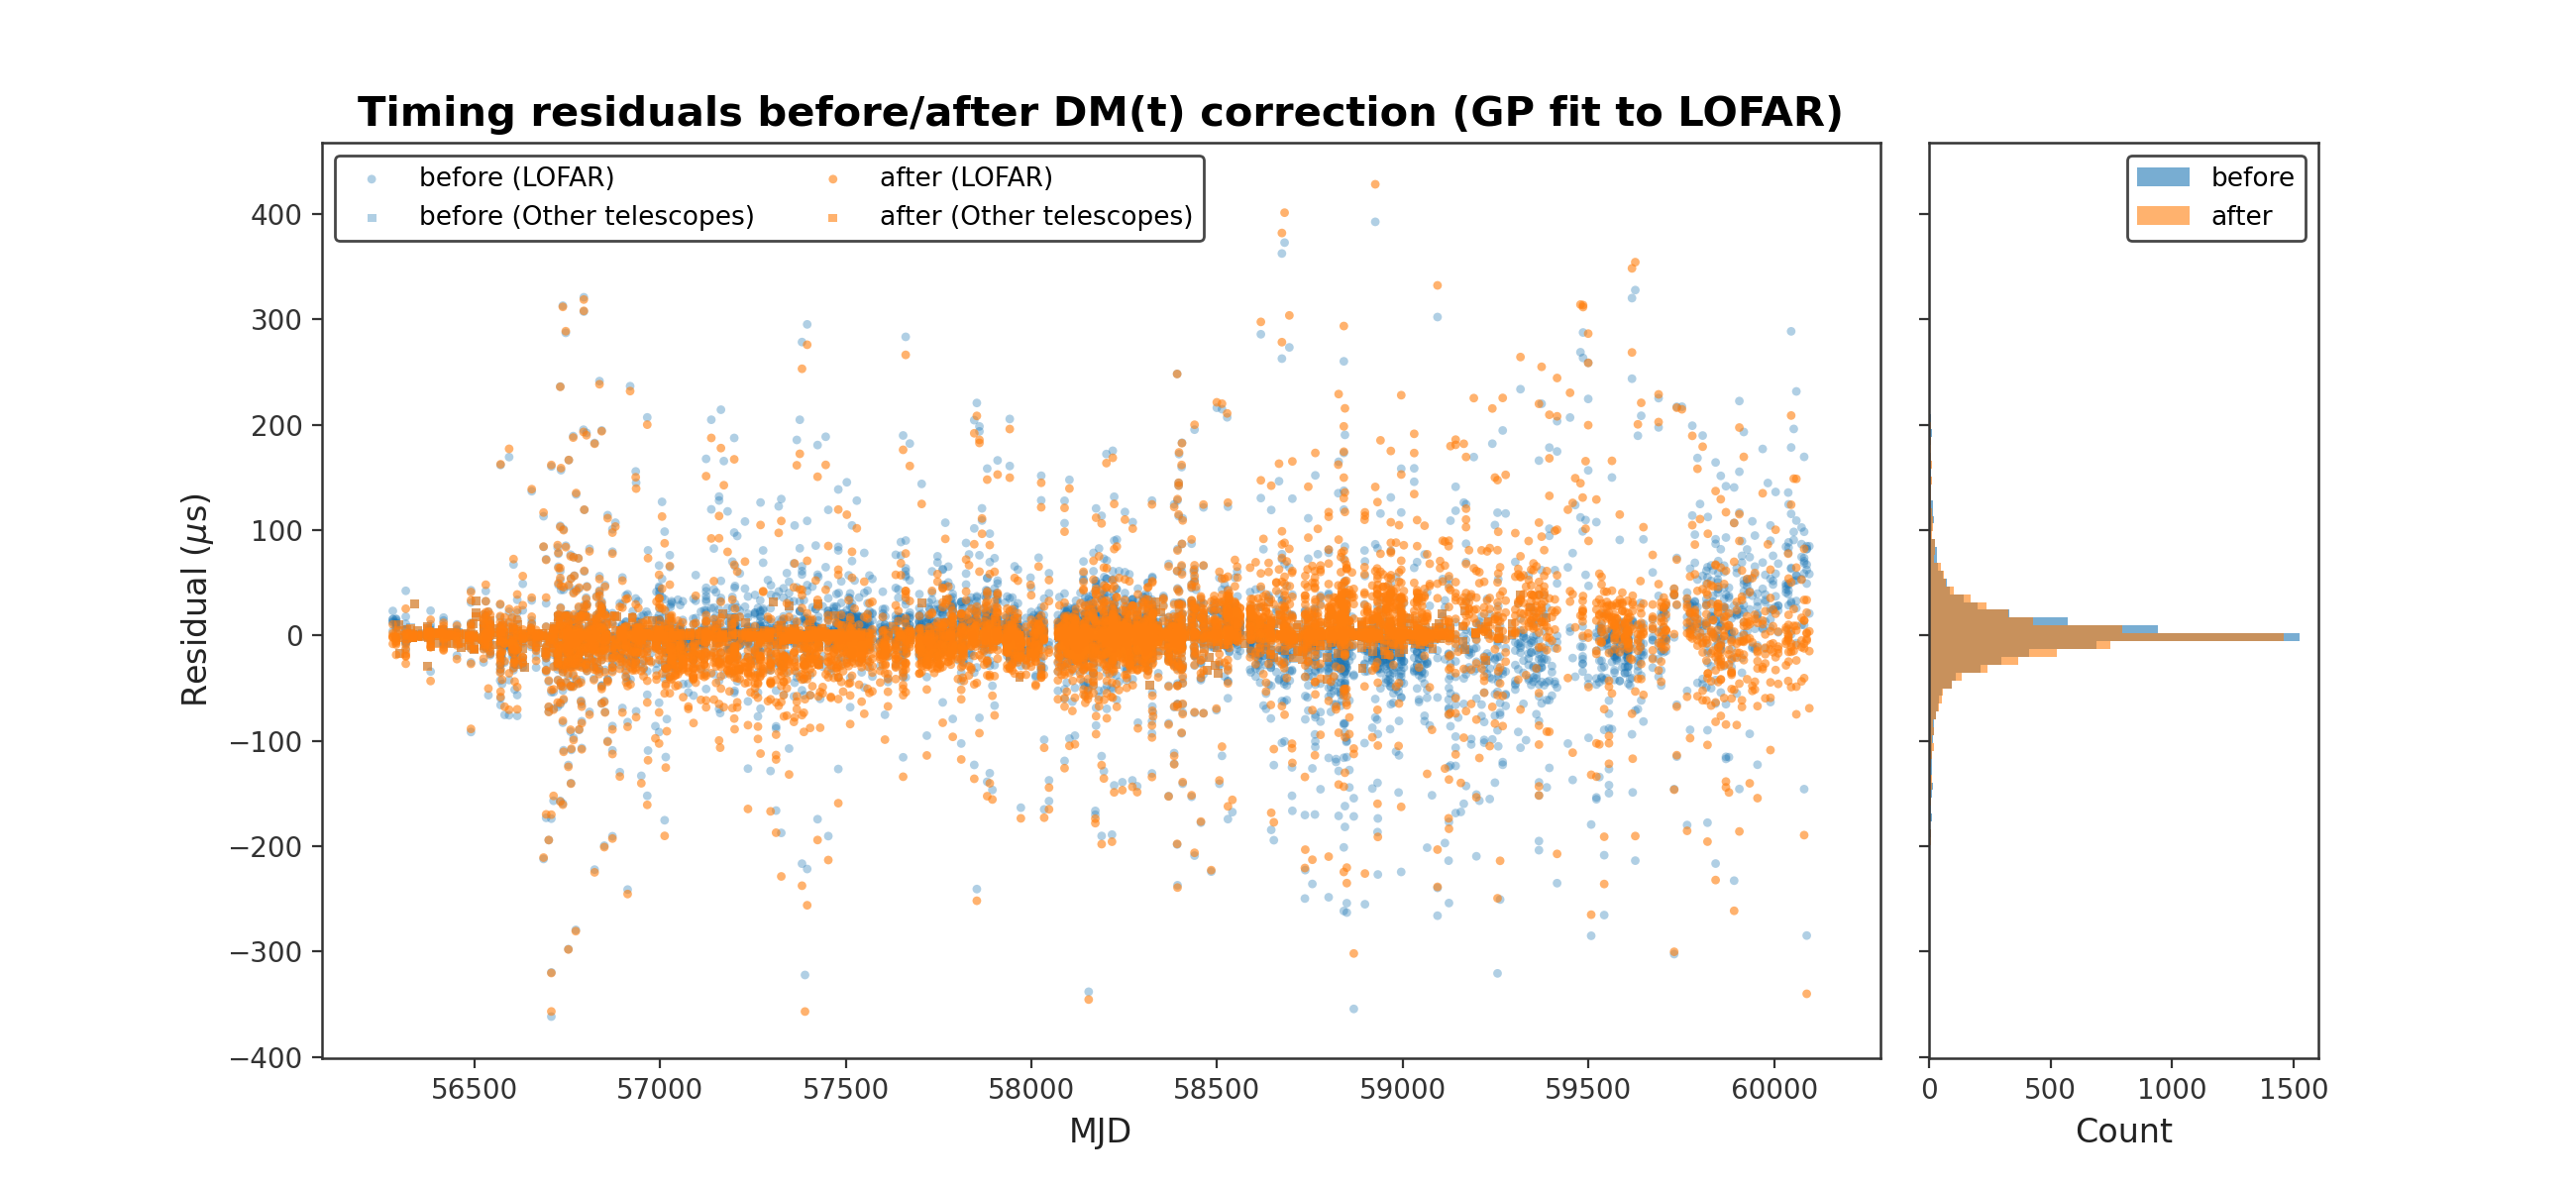
\includegraphics[width=0.8\textwidth]{../J1640+2224/dm_correction_out/residuals_pre_post.png}
\end{center}

\subsection{Noise-model comparisons}

\colorkeytable{J1640+2224}

\cmpjoint{../plot_output/compare/J1640+2224.pdf}{highfreq\_corrected: rnonly vs dmrn}
\cmpjoint{../plot_output/compare/J1640+2224_lofaronly_corrected_rnonly_vs_dmrn.pdf}{lofaronly\_corrected: rnonly vs dmrn}
\cmpjoint{../plot_output/compare/J1640+2224_corrected_dmrn_3way.pdf}{corrected, dmrn: highfreq vs lofaronly vs combined}
\cmpone{../plot_output/compare/J1640+2224_corrected_rnonly_3way.pdf}{corrected, rnonly: highfreq vs lofaronly vs combined}
\cmpjoint{../plot_output/compare/J1640+2224_uncorrected_vs_corrected.pdf}{combined: uncorrected vs corrected (dmrn)}
\cmpjoint{../plot_output/compare/J1640+2224_lofaronly_corr_vs_uncorr_dmrn.pdf}{lofaronly: corrected vs uncorrected (DM+RN)}
\cmpone{../plot_output/compare/J1640+2224_lofaronly_corr_vs_uncorr_rnonly.pdf}{lofaronly: corrected vs uncorrected (RN only)}
\cmpjoint{../plot_output/compare/J1640+2224_rnonly-corrected_vs_dmrn-uncorrected.pdf}{combined\_corrected:rnonly vs combined\_uncorrected:dmrn}
\cmpjoint{../plot_output/compare/J1640+2224_lofaronly_uncorrected_rnonly_vs_dmrn.pdf}{lofaronly\_uncorrected: rnonly vs dmrn}
\cmpone{../plot_output/compare/J1640+2224_rnonly_highfreqU_vs_lofaronlyU_vs_combinedU.pdf}{RN only, uncorrected: highfreq vs lofaronly vs combined}

\subsection{DM(t): GP reconstruction vs epoch-wise}
\cmpwide{../plot_output/compare/J1640+2224_dm_timeseries_ew_vs_gp.pdf}{combined\_corrected:dmrn DM GP vs the original epoch-wise curve}

\subsection{Interpretation}

J1640+2224 is the most informative of the three. In both
\emph{combined\_uncorrected:dmrn} and \emph{highfreq\_corrected:rnonly}, the
red-noise posterior is essentially unconstrained --- it rails against the
low-$\gamma$ edge of the prior with no clear peak, i.e.\ no real achromatic
signal is detected in either case. Yet in \emph{combined\_corrected:rnonly}
a well-determined red-noise peak appears at $\gamma\approx5$--$6$. Since
that peak only shows up once LOFAR is in the dataset \emph{and} there is no
DM GP to catch chromatic power, the most likely reading is that it is not
genuine broadband red noise but DM-like residual power leaking into the
achromatic channel --- i.e.\ the correction has not (yet) fully removed the
chromatic structure this pulsar's LOFAR data carries.

The three-way station split shows this is not simply \emph{lofaronly}'s own
signal bleeding through unchanged: under \emph{rnonly}, \emph{lofaronly}
alone finds its own well-constrained but \emph{different} peak
($\gamma\approx2$), while \emph{combined}'s peak sits at an even
\emph{higher} $\gamma$ than either sub-component on its own --- a value
neither \emph{highfreq} nor \emph{lofaronly} individually produce. Once a DM
GP is added (\emph{dmrn}), the ranking flips: \emph{combined} and
\emph{highfreq} both become essentially unconstrained, while
\emph{lofaronly}'s own red noise stays sharply peaked at
$\gamma\approx1.5$--$2$ regardless. This non-additivity --- \emph{combined}
is not a blend of its parts, and which station subset ``wins'' flips
depending on whether a DM GP is present --- is itself evidence that neither
an achromatic-only nor a DM+achromatic fit is cleanly separating genuine
broadband red noise from residual chromatic structure here. At the
\emph{lofaronly} level alone, however, the simple corrected-vs-uncorrected
comparison with no DM GP shows substantial overlap --- unlike J1012+5307 ---
suggesting the \emph{combined\_corrected:rnonly} anomaly specifically
depends on \emph{mixing} LOFAR with high-frequency stations, not on
anything intrinsic to the LOFAR band by itself. The same DM-GP reassignment
degeneracy as J1012+5307 is nonetheless present within \emph{lofaronly}
too: adding a DM GP leaves corrected red noise unchanged while uncorrected
goes fully unconstrained, with the DM GP cleanly detecting a signal
($\gamma\approx2$, well-localized) only in the uncorrected data. The
three-way \emph{rnonly} split among the three \emph{uncorrected} station
sets again gives three mutually exclusive, well-determined peaks.

\section{J1744$-$1134}
\label{sec:J1744}

\subsection{Epoch-wise DM(t) correction}
\begin{center}
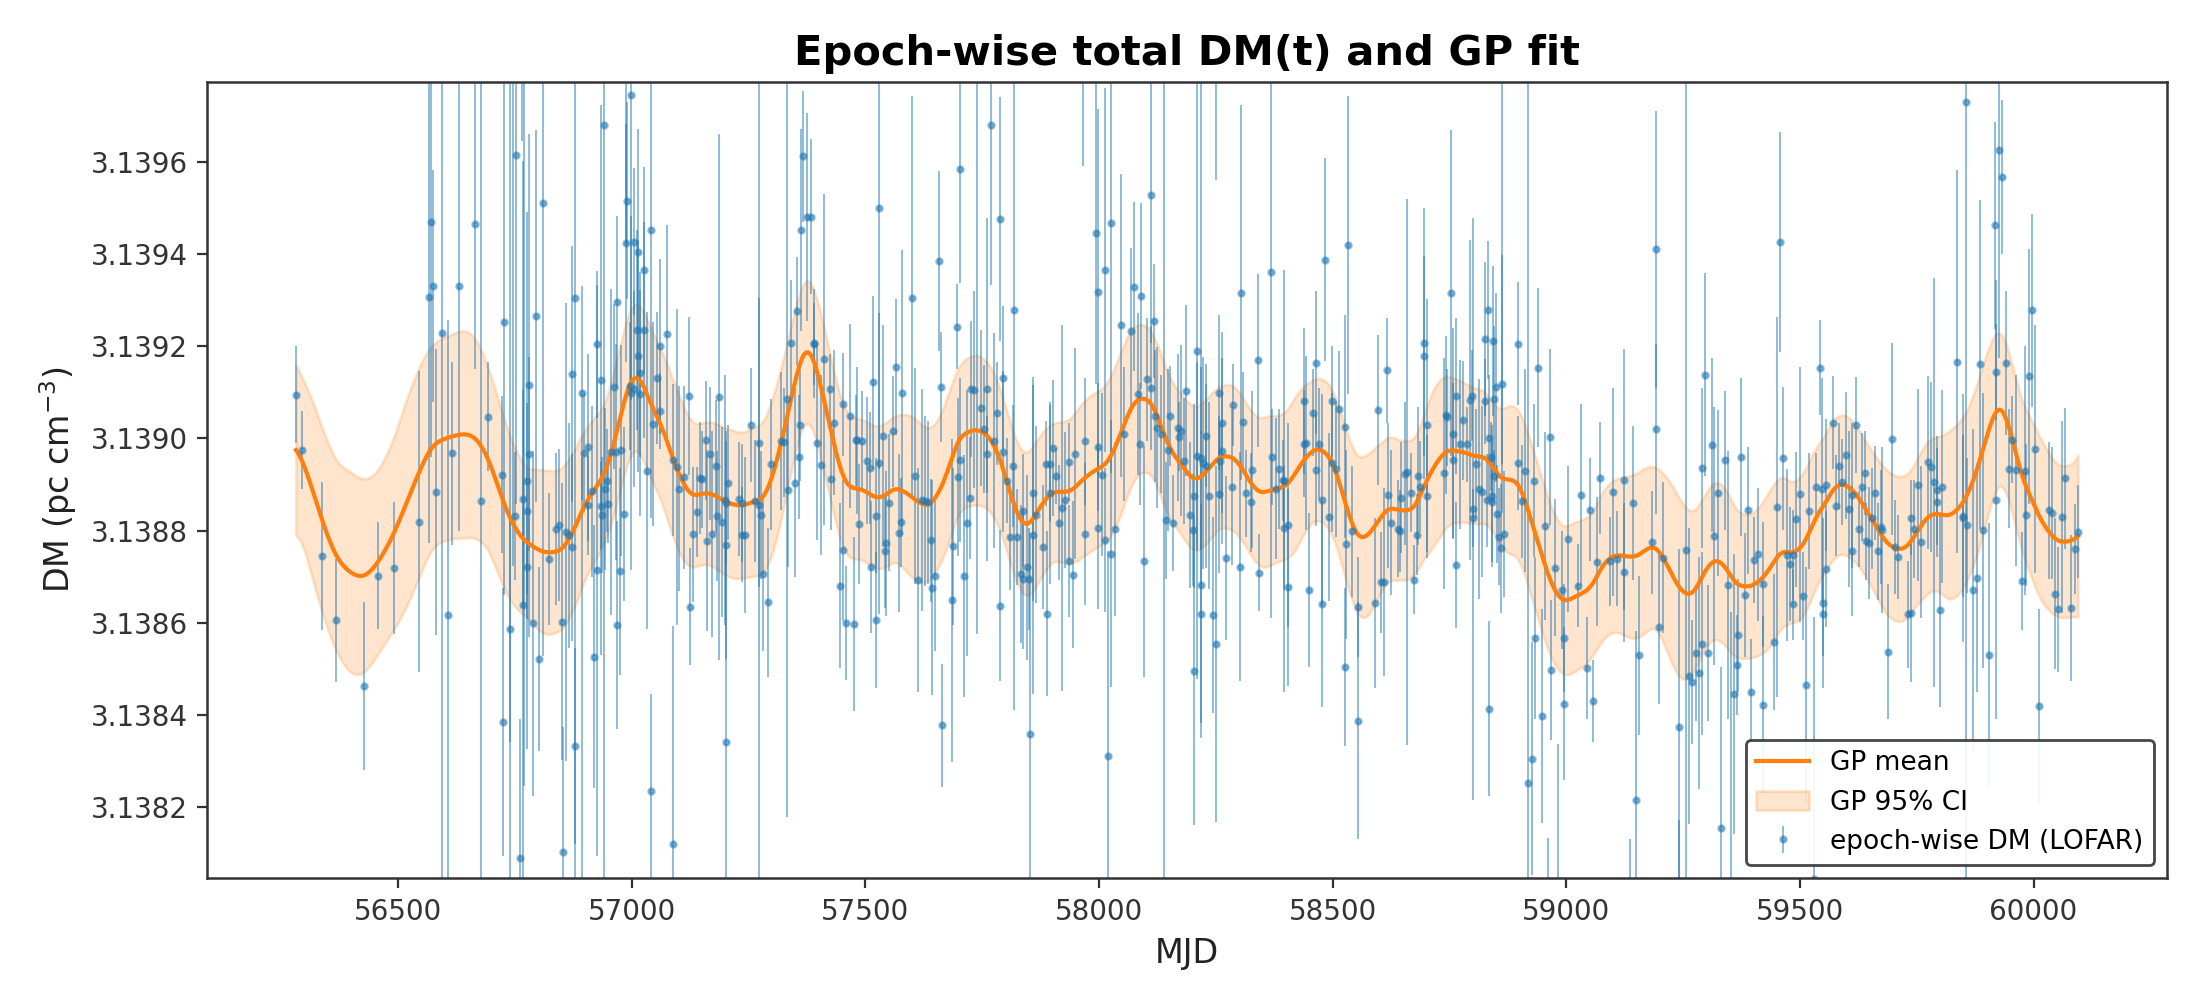
\includegraphics[width=0.8\textwidth]{../J1744-1134/dm_correction_out/dm_timeseries.png}
\end{center}

\subsection{Effect on residuals}
\begin{center}
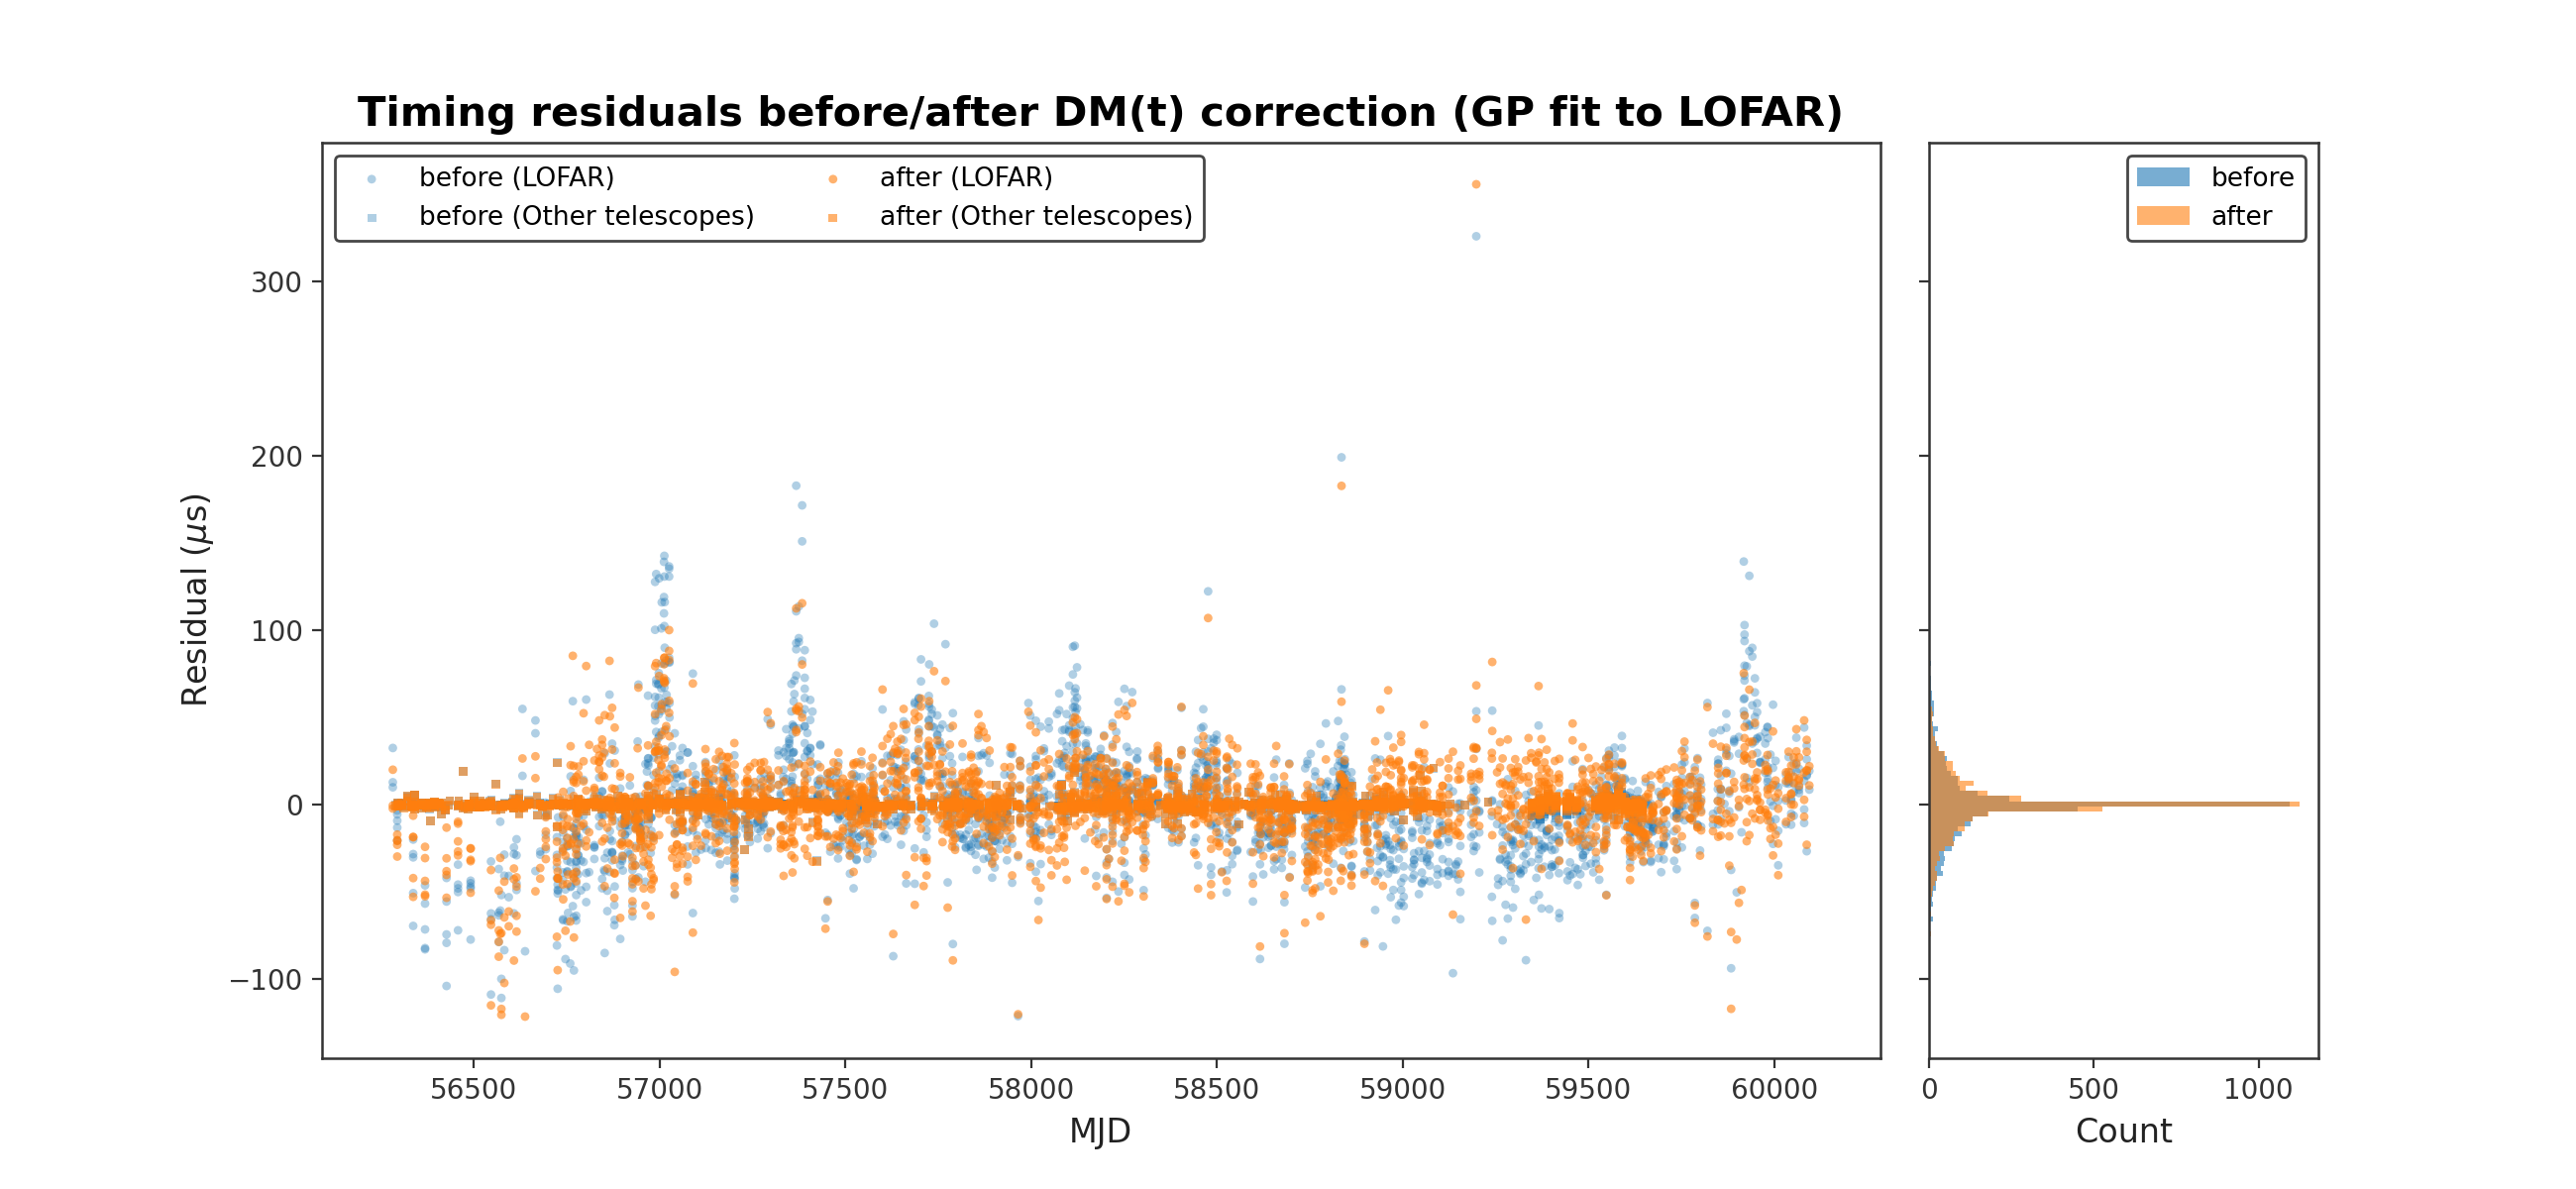
\includegraphics[width=0.8\textwidth]{../J1744-1134/dm_correction_out/residuals_pre_post.png}
\end{center}

\subsection{Noise-model comparisons}

\colorkeytable{J1744-1134}

\cmpjoint{../plot_output/compare/J1744-1134.pdf}{highfreq\_corrected: rnonly vs dmrn}
\cmpjoint{../plot_output/compare/J1744-1134_lofaronly_corrected_rnonly_vs_dmrn.pdf}{lofaronly\_corrected: rnonly vs dmrn}
\cmpjoint{../plot_output/compare/J1744-1134_corrected_dmrn_3way.pdf}{corrected, dmrn: highfreq vs lofaronly vs combined}
\cmpone{../plot_output/compare/J1744-1134_corrected_rnonly_3way.pdf}{corrected, rnonly: highfreq vs lofaronly vs combined}
\cmpjoint{../plot_output/compare/J1744-1134_uncorrected_vs_corrected.pdf}{combined: uncorrected vs corrected (dmrn)}
\cmpjoint{../plot_output/compare/J1744-1134_lofaronly_corr_vs_uncorr_dmrn.pdf}{lofaronly: corrected vs uncorrected (DM+RN)}
\cmpone{../plot_output/compare/J1744-1134_lofaronly_corr_vs_uncorr_rnonly.pdf}{lofaronly: corrected vs uncorrected (RN only)}
\cmpjoint{../plot_output/compare/J1744-1134_rnonly-corrected_vs_dmrn-uncorrected.pdf}{combined\_corrected:rnonly vs combined\_uncorrected:dmrn}
\cmpjoint{../plot_output/compare/J1744-1134_lofaronly_uncorrected_rnonly_vs_dmrn.pdf}{lofaronly\_uncorrected: rnonly vs dmrn}
\cmpone{../plot_output/compare/J1744-1134_rnonly_highfreqU_vs_lofaronlyU_vs_combinedU.pdf}{RN only, uncorrected: highfreq vs lofaronly vs combined}

\subsection{DM(t): GP reconstruction vs epoch-wise}
\cmpwide{../plot_output/compare/J1744-1134_dm_timeseries_ew_vs_gp.pdf}{combined\_corrected:dmrn DM GP vs the original epoch-wise curve}

\subsection{Interpretation}

J1744$-$1134 is the one pulsar where the correction behaves as intended: the
red-noise posterior overlaps substantially across all three tests ---
\emph{combined\_corrected:rnonly} vs \emph{combined\_uncorrected:dmrn},
and \emph{combined\_corrected:rnonly} vs \emph{highfreq\_corrected:rnonly}
--- with no strong dependence on whether LOFAR is included or whether DM is
modelled explicitly. The caveat: J1744$-$1134 is close to the ecliptic, so
part of what the epoch-wise correction measures and removes near solar
conjunction may be solar-wind signal rather than pure interstellar DM(t).
The clean agreement seen here is consistent with the correction working,
but is not on its own proof that it is working \emph{for the right reason}.

The three-way station split confirms this directly: under both
\emph{rnonly} and \emph{dmrn}, \emph{combined} tracks \emph{highfreq}
closely, even though \emph{lofaronly} alone finds a distinct peak in each
case --- a higher-amplitude red noise under \emph{rnonly}, and a DM GP
offset in amplitude (though not spectral index) from \emph{highfreq}'s own
under \emph{dmrn}. In other words, LOFAR's own slightly different
preference is simply outweighed once merged with the more numerous
high-frequency data here, rather than \emph{combined} inheriting it the way
it does for J1012+5307 and J1640+2224. Unlike those two pulsars, the
corrected-data DM GP does \emph{not} fully rail to zero amplitude when
isolated to \emph{lofaronly} alone; it retains a modest, well-localized
peak ($\gamma<1$, $\log_{10}A\approx-14$), distinct from but closer to the
uncorrected DM GP's own peak than in either other pulsar. This is
consistent with the ecliptic-proximity caveat already raised: some
residual, DM-like power survives the correction here, plausibly solar-wind
signal that NE\_SW$\to$0 alone does not remove. The three-way \emph{rnonly}
split among the three \emph{uncorrected} station sets still shows three
disjoint peaks ordered by frequency band, confirming that even in this
best-behaved case, an achromatic-only fit on uncorrected data is sensitive
to which stations are included --- the correction's job is still necessary
here, it is simply more complete than for the other two pulsars.


\section{Cross-pulsar synthesis}

A consistent pattern emerges across the red-noise comparisons (Sections
\ref{sec:J1012}--\ref{sec:J1744}): whenever (a) the dataset includes LOFAR
(\emph{combined}, as opposed to \emph{highfreq}) \emph{and} (b) the noise
model has no explicit DM GP (\emph{rnonly}), the recovered red-noise
amplitude and spectral index shift, often with the unconstrained-RN case
(prior railing at low $\gamma$) appearing in whichever side is \emph{not}
exposed to LOFAR's chromatic sensitivity. This is exactly what you would
expect if some chromatic signal remains unmodelled when nothing is there to
catch it.

\textbf{J1744$-$1134} behaves as the correction is intended to: the
corrected-dataset red noise is consistent whether or not a DM GP is present,
and whether or not LOFAR is included. Its proximity to the ecliptic means
this should be read with some caution, though --- part of what the epoch-wise
correction absorbs there may be solar-wind signal rather than pure
interstellar DM(t), so the clean agreement is not unambiguous evidence that
the correction is doing only what it is meant to.

\textbf{J1012+5307} and \textbf{J1640+2224} show the opposite: the red noise
recovered from the \emph{combined} dataset (or from \emph{rnonly}, which has
no DM GP to intercept chromatic signal) is systematically different from the
\emph{highfreq}-only / DM-GP-separated case. For J1640+2224 in particular,
the red noise is essentially unconstrained in \emph{highfreq\_corrected:rnonly}
and in \emph{combined\_uncorrected:dmrn}, but well-determined in
\emph{combined\_corrected:rnonly} --- suggesting that what shows up as "red
noise" there is more likely uncorrected chromatic (DM-like) power leaking
into the achromatic channel than genuine broadband red noise.

The DM(t) time-domain reconstructions (one subsection per pulsar) test this
directly for the corrected, combined dataset: if the correction were
complete, the residual DM GP recovered on \emph{already-corrected} data
should show no resemblance to the original epoch-wise curve it was
corrected with.

\end{document}
